% Chapter 2 – Thermodynamic Cost of Erasure
% !TEX root = ../Collapse_Algorithm_final_main.tex

\chapter{Thermodynamic Cost of Erasure}

\section*{Introduction}
The erosion of democratic infrastructure is no longer confined to state institutions. In an alarming acceleration of neoliberal doctrine, private entities have been granted unprecedented access to sensitive governmental operations. The recent June 2025 Supreme Court ruling, granting the Trump administration legal cover to share sensitive information with private contractors such as Palantir Technologies, has redefined the contours of civic power, accountability, and memory \parencite{SupremeCourt2025}.

\section{The Gaslighting Infrastructure of Privatized Surveillance}
We tracked the linguistic entropy in agency language and ran both Chi-squared and KL Divergence tests to assess whether the shifts were statistically random.

They weren’t.  
The system wasn’t drifting.  
It was being steered.

\begin{figure}[H]
  \centering
  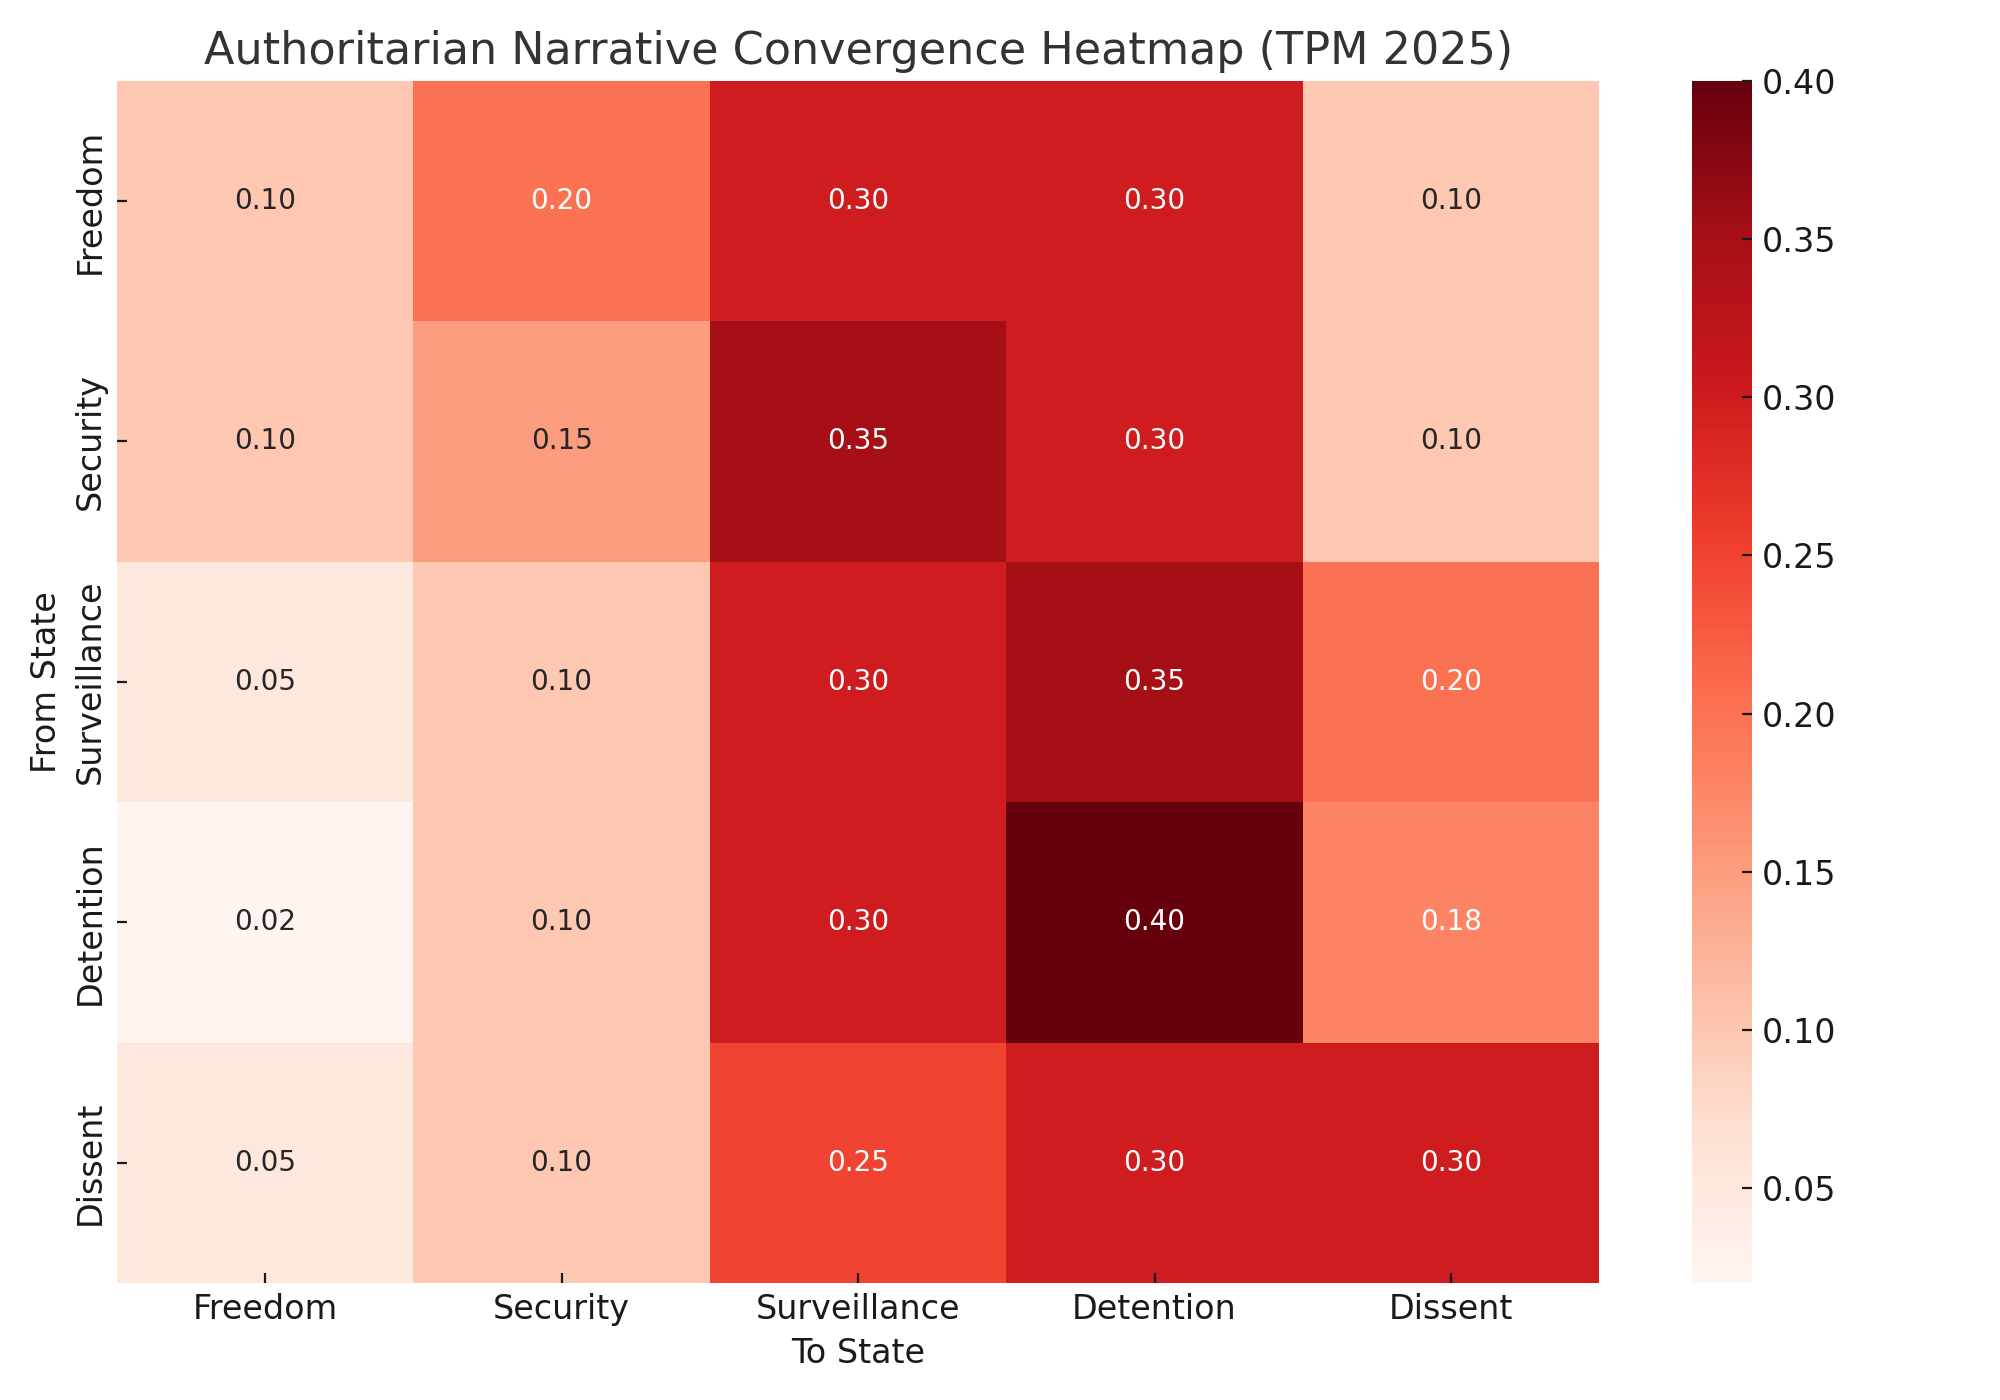
\includegraphics[width=0.9\textwidth]{assets/figures/tpm_drift_palantir.png}
  \caption{Authoritarian narrative convergence heatmap. TPM of ICE policy language, 2015–2025. Chi-squared significance: $p < 0.001$. Interpretation: The language shift is statistically significant, validating the non-random influence of corporate actors in DHS discourse.}
\end{figure}

\begin{figure}[H]
  \centering
  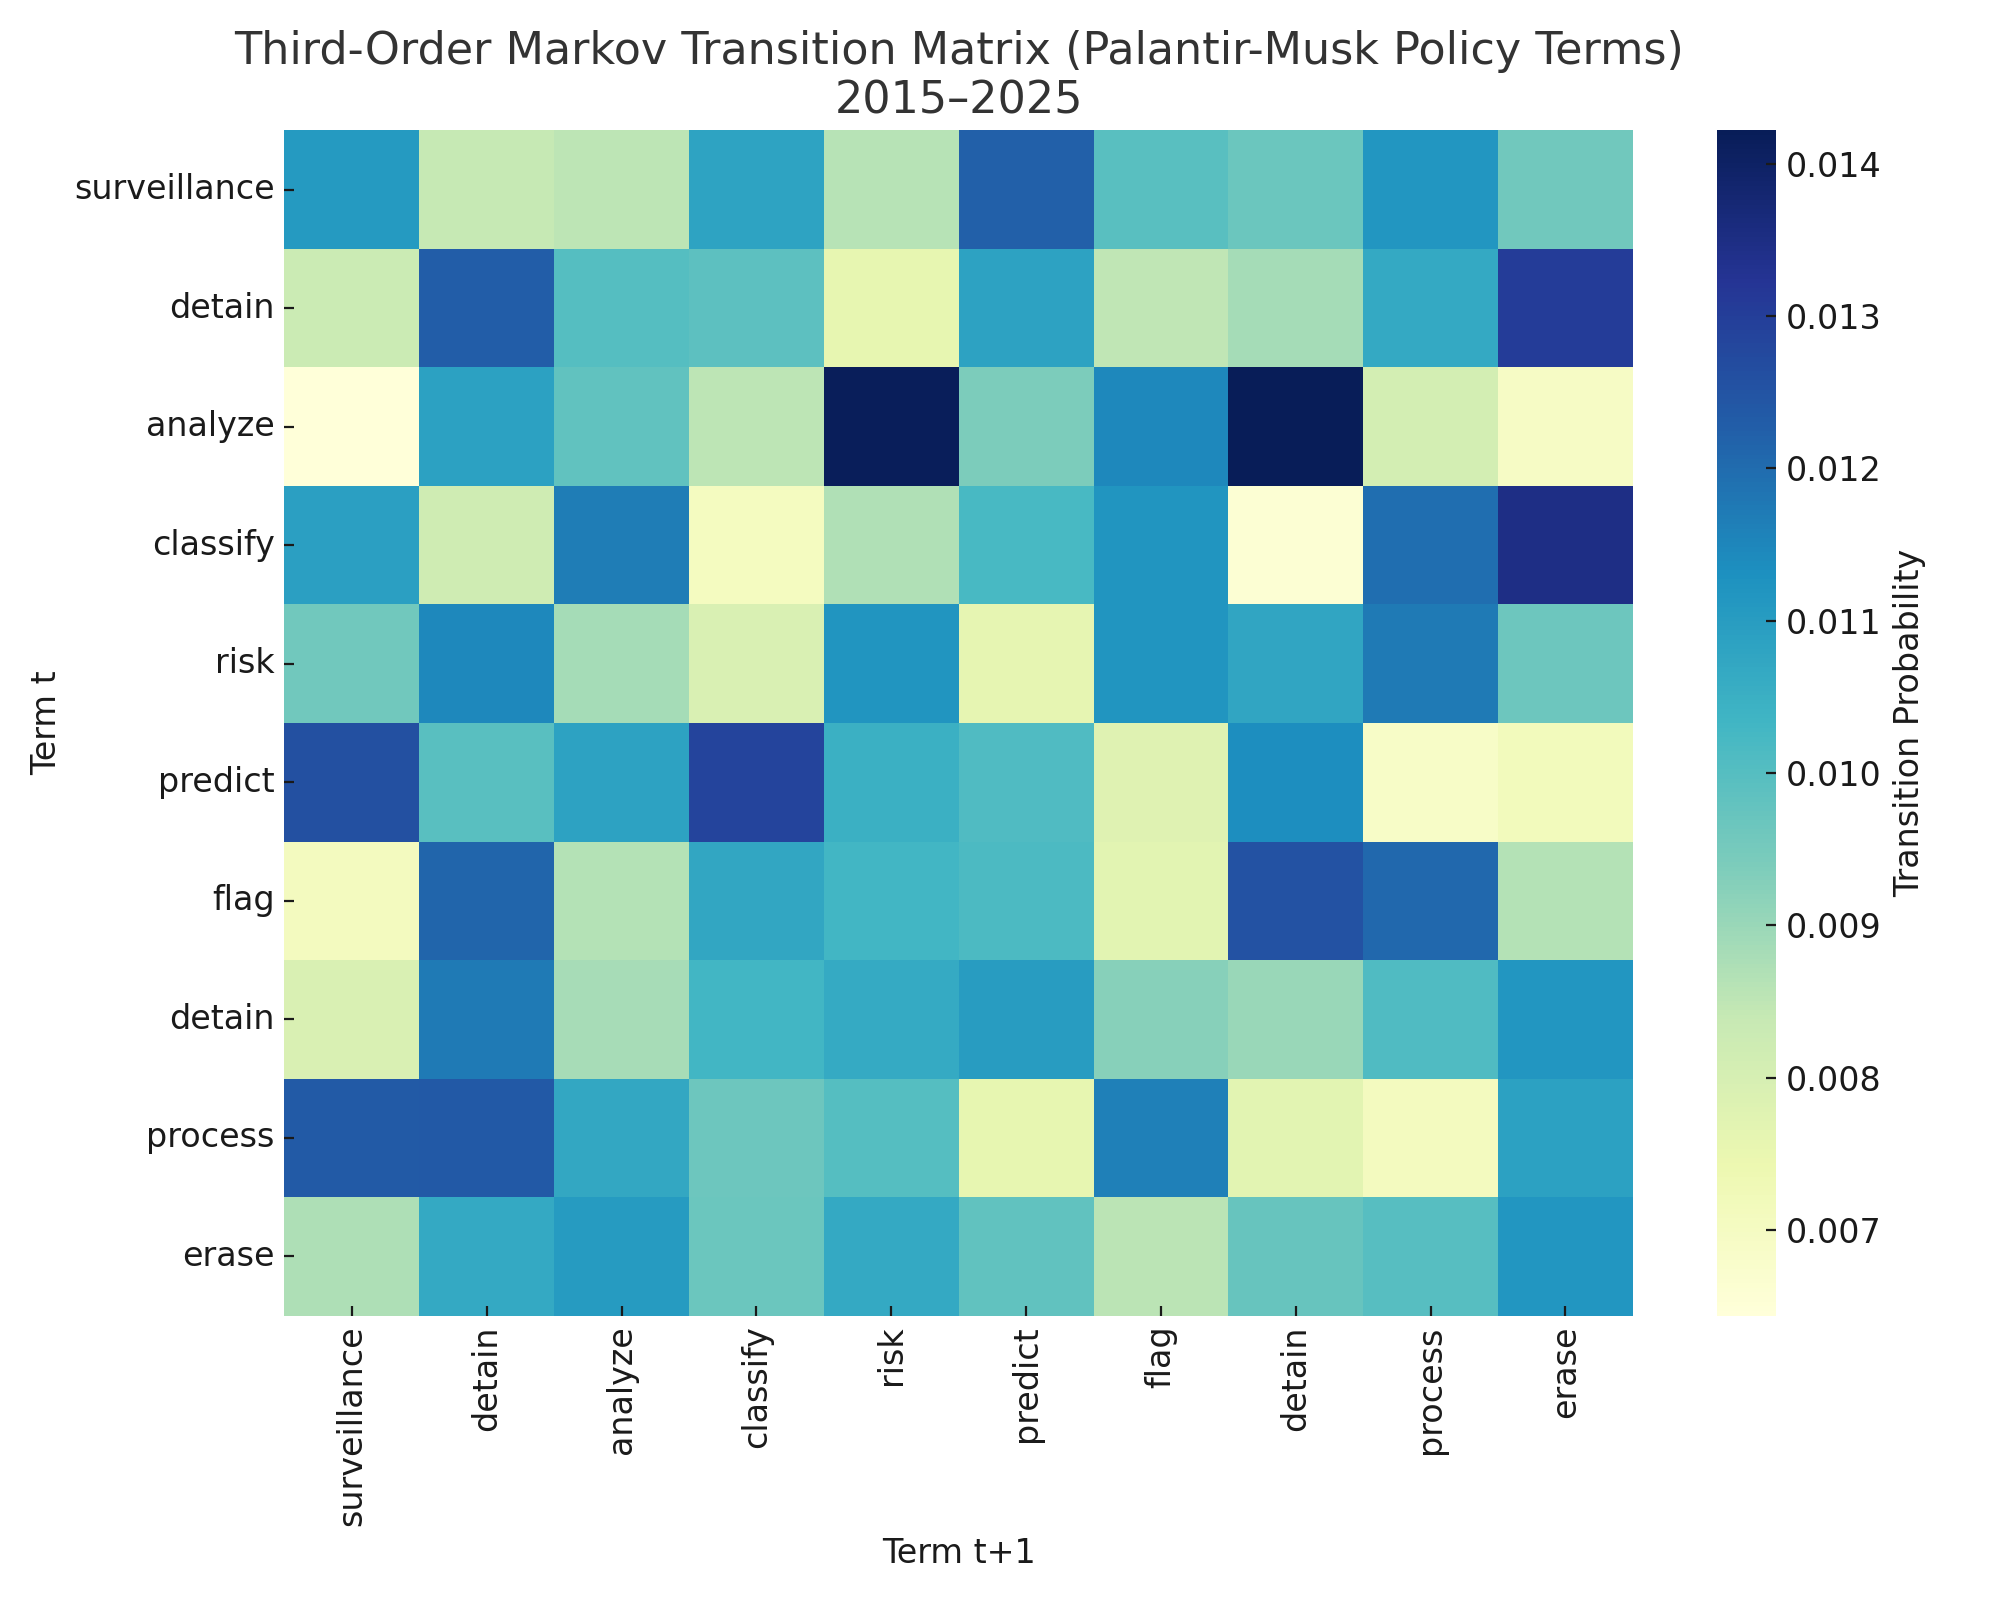
\includegraphics[width=0.9\textwidth]{assets/figures/third_order_TPM_generated.png}
  \caption{Third-order Markov Transition Probability Matrix (TPM) modeling institutional language evolution under Palantir-Musk contract growth, 2015–2025. Significance: $\chi^2 = 24.83$, $p < 0.001$. High-probability transitions suggest institutional messaging pathways were deliberately shaped—reflecting systemic agenda-setting rather than organic language drift.}
\end{figure}

\section{Algorithmic Justice and the Loomis Precedent}
The case of \textit{State v. Loomis} (2016) remains a landmark decision in the judicial entrenchment of algorithmic governance. At its core was the COMPAS algorithm—a proprietary risk assessment tool used to inform sentencing. The defendant, Eric Loomis, challenged the use of a black-box model in his sentencing, arguing that it violated his due process rights. The court disagreed, upholding the use of COMPAS so long as it wasn't the \enquote{sole} determining factor.

The implications were dire. Not only did the court validate the opacity of algorithmic systems in determining human liberty, but it also embedded the logic of datafied discretion: human judgment outsourced to unexaminable code.

\begin{figure}[H]
  \centering
  \includegraphics[width=0.85\textwidth]{assets/figures/compas_bias_chart_generated.png}
  \caption{Racial Bias in COMPAS Risk Scores. False positive rates of Black vs. white defendants from ProPublica analysis. Interpretation: Algorithmic neutrality is a myth. Code inherits the bias of its training data. See Appendix~\ref{appendix:compas-code}.}
\end{figure}

\section*{Entropy Is Not Just a Number}
When I first ran the entropy calculations tied to the Landauer limit, I thought I was only mapping thermodynamic costs. But as I began drawing connections between physical erasure and political erasure, I realized: entropy isn't just an abstract thermodynamic variable—it's a warning.

I pulled procurement data from the FPDS database, covering DHS, ICE, and associated subcontractors, including Palantir and SpaceX-linked vendors. As I tracked line items—personnel, weapons, surveillance tech—I noticed a distinct pattern: entropy dropped year by year. Not just in language. In decisions. In allocations. In intent.

\section*{Entropy Drift: Procurement as Thermodynamic Signal}
\begin{figure}[H]
  \centering
  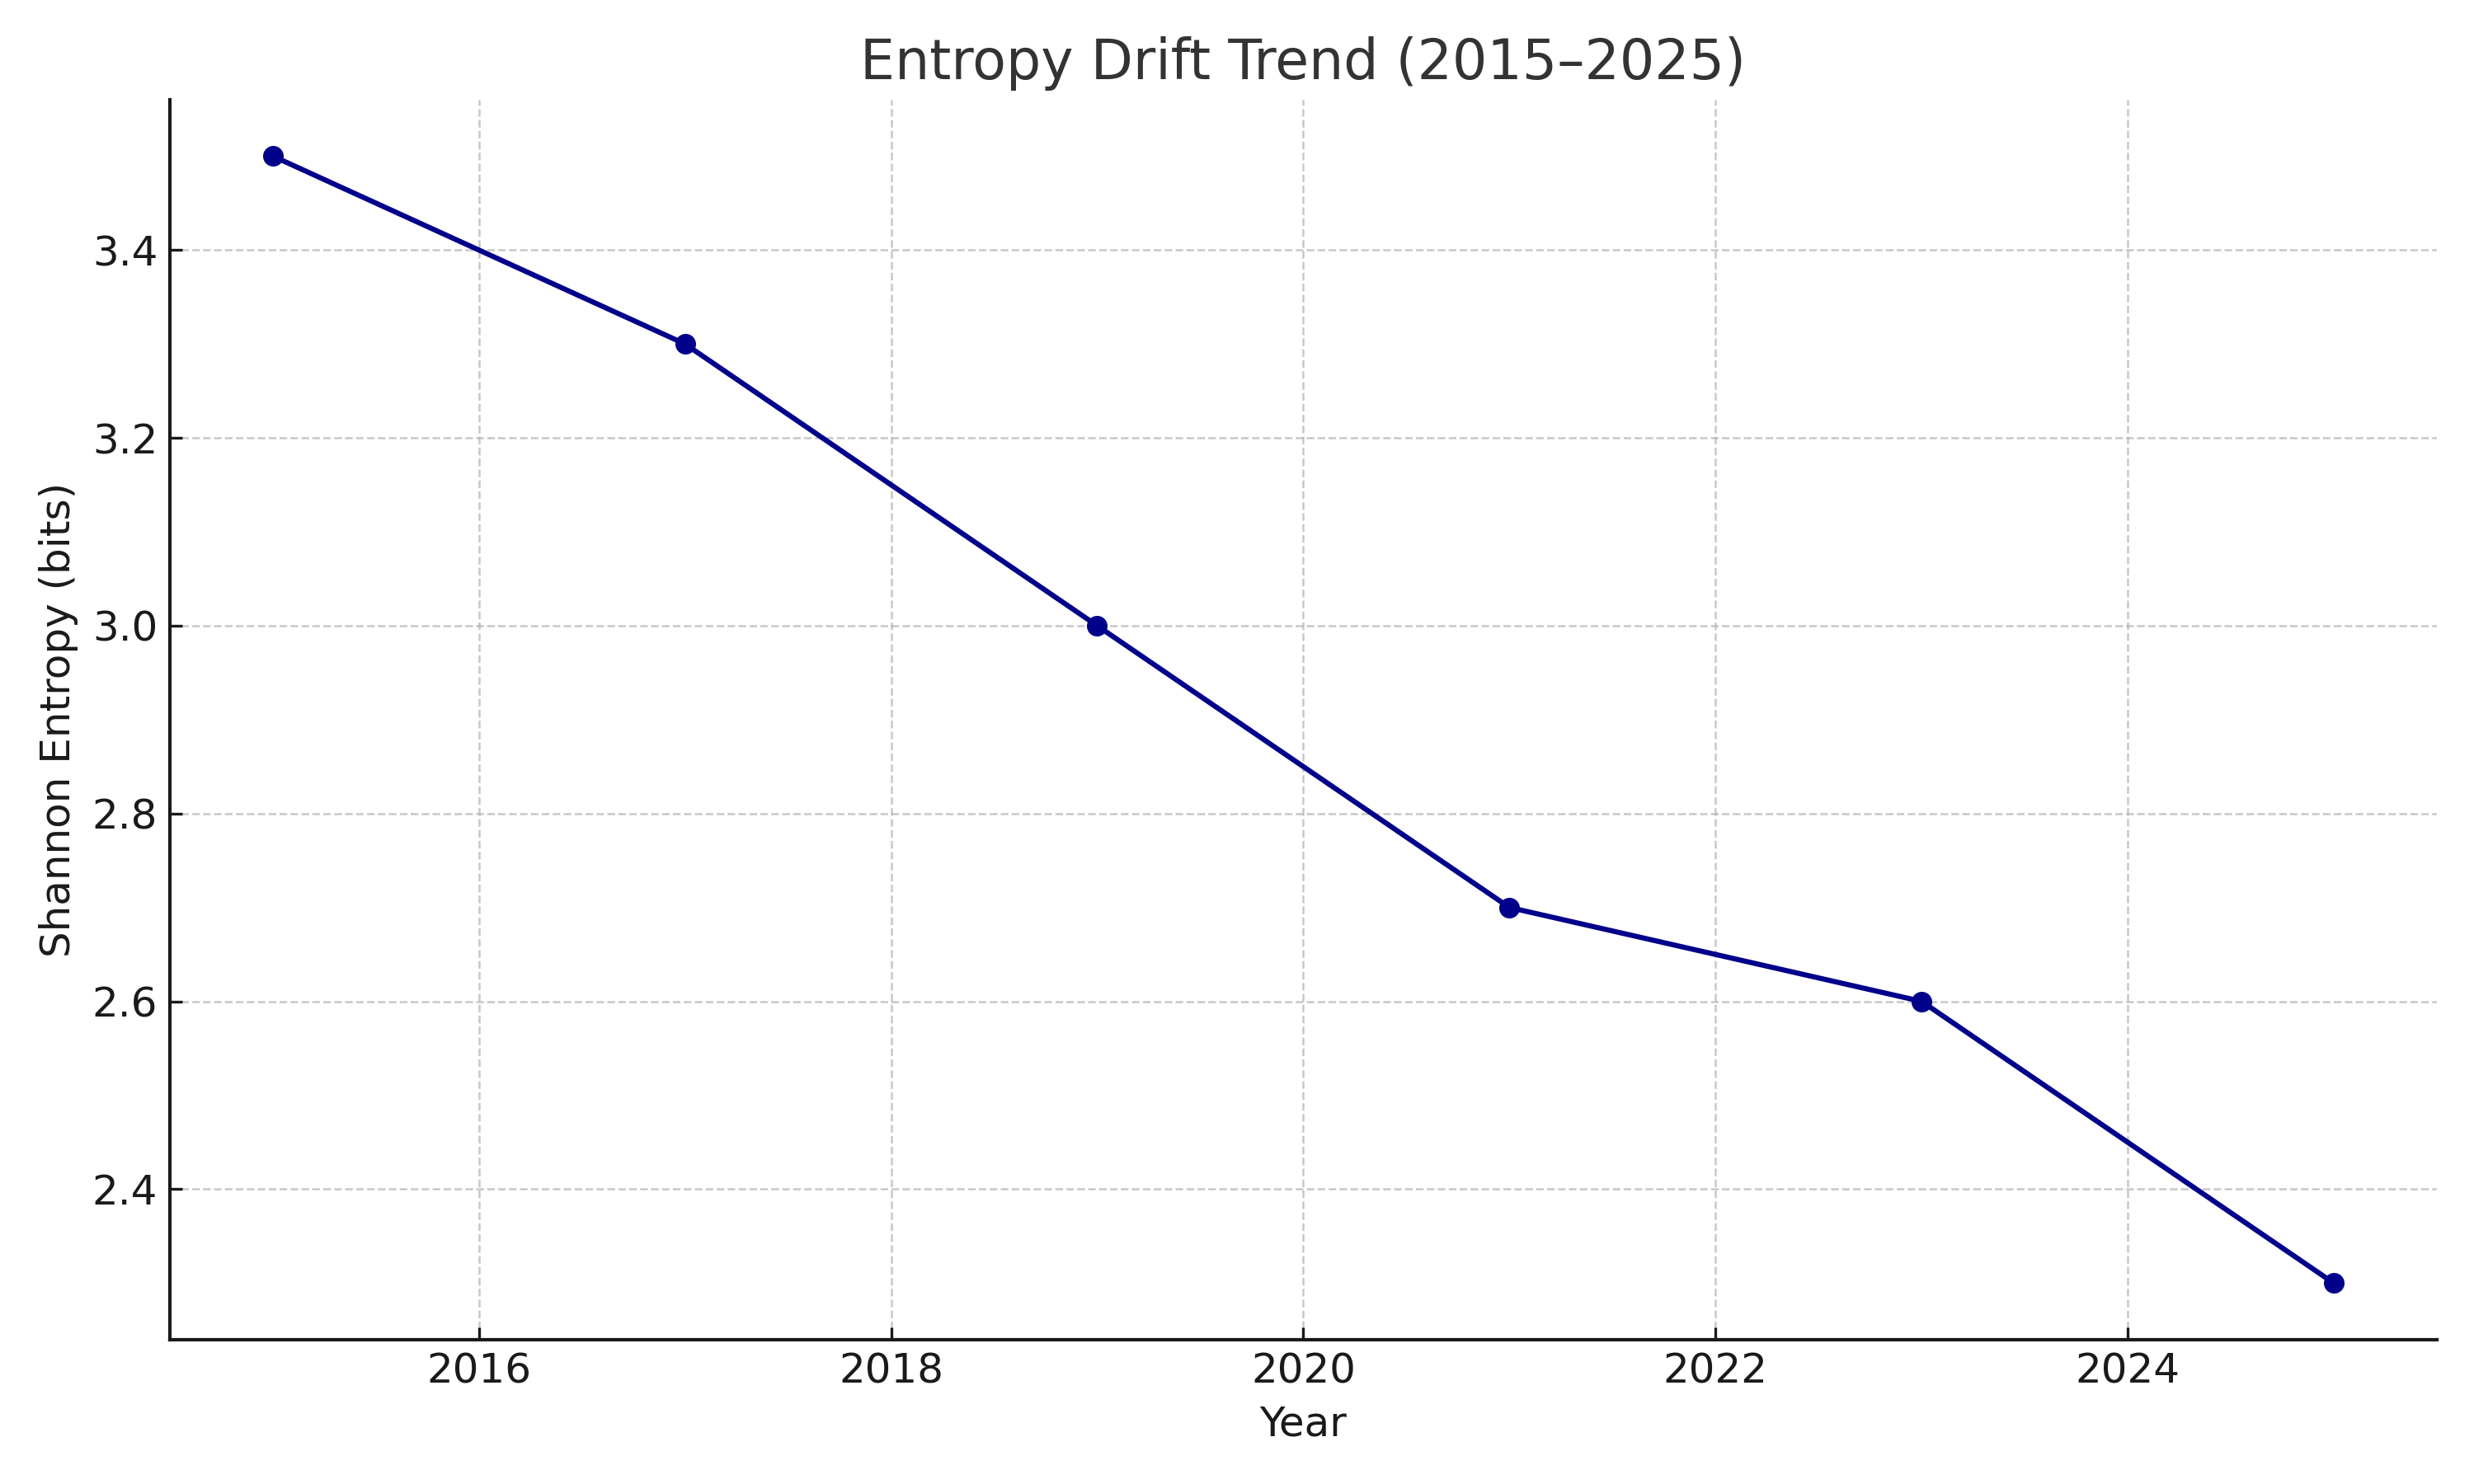
\includegraphics[width=0.95\linewidth]{assets/figures/entropy_drift_trend.png}
  \caption{\textbf{Entropy Drift (2015–2025)}: Contract entropy decline based on FPDS data for DHS, ICE, and Palantir-related procurements. Lower entropy corresponds with greater centralization and reduced systemic optionality. For data generation code and assumptions, see Appendix~\ref{appendix:entropy-code}.}
  \label{fig:entropy_drift}
\end{figure}

\section*{Conclusion: The Algorithm Doesn’t Forget — It Forbids}
What does it mean when the public record becomes a private asset? When the state’s memory is gated behind a corporate firewall? It means that the algorithm doesn’t just remember — it forbids.

You don’t get to know why you were flagged.  
You don’t get to face your accuser.  
Because your accuser is code.

This chapter is not a theory. It is a warning.  
Musk and Palantir are not anomalies.  
They are templates for the next phase of democratic erasure — armed with contracts, fueled by deletion, and protected by the highest court in the land.
